\documentclass[a4paper,12pt,oneside]{article}
\usepackage{amsmath}
%\usepackage{mathtools}
\usepackage{caption}
\usepackage{mathptmx}
\usepackage{fixltx2e}
\usepackage{graphicx}
\usepackage[margin=1.0in]{geometry}
\usepackage{float}
\usepackage{setspace}
\usepackage{chngcntr}
\usepackage{fancyhdr}
\pagestyle{fancy}
\fancyhf{}
\rfoot{\thepage}
%\renewcommand{\headrulewidth}{0.0pt}
%\renewcommand{\footrulewidth}{0.0pt}

\begin{document}
\thispagestyle{empty}
%\pagenumbering{gobble}
\begin{center}

\large{\textbf{{APPLICATION OF SENTIMENT ANALYSIS TO LANGUAGE LEARNING}}}
\setlength{\baselineskip}{1.5\baselineskip}
\\
\vspace{5mm}
\textbf{SEMINAR REPORT}

Submitted in the partial fulfilment of the award of the degree
of
\\
\textbf{Bachelor of Technology}
\\
in
\\
\textbf{Computer Science \& Engineering}
\\
of
\\
\textbf{APJ Abdul Kalam Technological University}
\\
by
\\
\textbf{GEORGY JOSE VILAVINAL}
\\
\vspace{5mm}
\begin{figure}[H]
\centering

\includegraphics{ceclogo.png}
\end{figure}
\textbf{November, 2018}
\vspace{8mm}
\\
Department of Computer Engineering
\\
College of Engineering, Chengannur, Kerala -689121
\\
Phone: (0479) 2454125, 2451424; Fax: (0479) 2451424
\\
\end{center}

\newpage
\thispagestyle{empty}
\begin{center}
\setlength{\baselineskip}{1.5\baselineskip}
{\large\textbf{COLLEGE OF ENGINEERING, CHENGANNUR}}
\\
{\large\textbf{KERALA}}
\\
\begin{figure}[H]
\centering

\includegraphics{ceclogo.png}
\end{figure}
\setlength{\baselineskip}{1.5\baselineskip}
\textbf{Department of Computer Engineering}
\\
\textbf{CERTIFICATE}
\\
This is to certify that the seminar entitled
\\
\textbf{APPLICATION OF SENTIMENT ANALYSIS TO LANGUAGE LEARNING}
\\
Submitted by
\\
\textbf{GEORGY JOSE VILAVINAL}
\\
is a bonafide record of the work done by him.
\end{center}
\vspace{14ex}
%\textbf{Mrs.Sheeba}
\hspace{55ex}
%\textbf{Dr. Smitha Dharan}
\\
\vspace{2ex}
\hspace{0ex}
\textbf{
Co-ordinator}
\hspace{45ex}
\textbf{
Head of The Department}
\newpage
\pagenumbering{roman}
\renewcommand{\headrulewidth}{0.0pt}
\renewcommand{\footrulewidth}{0.0pt}
\begin{center}
\large{\textbf{ACKNOWLEDGEMENT}}
\end{center}
\vspace{6ex}
\setlength{\baselineskip}{1.5\baselineskip}
\paragraph{}
I am greatly indebted to \textbf{God Almighty} for being the guiding light throughout with his
abundant grace and blessings that strengthened me to do this endeavour with confidence.
\paragraph{}
I express my heartfelt gratitude towards \textbf{Dr. Jacob Thomas V.}, Principal, College
of Engineering Chengannur for extending all the facilities required for doing my seminar.
I would also like to thank \textbf{Dr. Smitha Dharan}, Head, Department of Computer
Engineering, for providing constant support and encouragement.
\paragraph{}
Now I extend my sincere thanks to my seminar co-ordinators \textbf{Ms. Shiny B}, Associate
Professor in Computer Engineering and \textbf{Ms. Angel Thomas} , Assistant
Professor in Computer Engineering for guiding me in my work and providing timely
advices and valuable suggestions.
\paragraph{}
Last but not the least, I extend my heartfelt gratitude to my parents and friends for
their support and assistance.	
\pagenumbering{gobble}

\newpage
\begin{center}
\large{\textbf{ABSTRACT}}
\end{center}
\vspace{4ex}
\paragraph{}
Emotion vocabulary has been studied in various disciplines, such as psychology, linguistics, and computational linguistics. Recently, it plays a requisite role in sentiment analysis or opinion mining. However, emotion vocabulary has not received considerable attention in second or foreign language learning. The insufficient pedagogical materials and inefficient tool support seem to provide little help for learners to master emotion words. The current study considers the application of sentiment analysis to language learning. \textbf{RESOLVE} is a context-aware emotion synonym suggestion system, which utilizing machine-learning techniques, the system is capable of suggesting synonymous emotion words appropriate to learners’ contexts. Importantly, the usage information of each emotion word, including scenario descriptions, definitions, and example sentences, is provided in order to help develop language learners’ vocabulary knowledge as well as help facilitate their word use. 
\paragraph{}
A pedagogical evaluation of the system’s effectiveness was conducted using a writing task and a survey questionnaire. The results indicate that the participants achieved substantial progress on emotion word use with the help of the proposed system. In particular, less proficient participants demonstrated greater improvements. Meanwhile, participants showed positive attitudes toward the tool support, as it helps them to have a better command of emotion words in their writings.
\setlength{\baselineskip}{1.0\baselineskip}
\newpage
\begin{center}
\tableofcontents
\end{center}

% List of Figures Page
% \newpage
% \thispagestyle{plain}
% \begin{center}
% \listoffigures
% \end{center}

\newpage
\rfoot{\thepage}
\lhead{\textit{Application of Sentiment Analysis to Language Learning}}
\lfoot{\textit{College of Engineering Chengannur}}
\rfoot{\thepage}
\renewcommand{\headrulewidth}{0.0pt}
\renewcommand{\footrulewidth}{0.0pt}
\renewcommand{\headrulewidth}{0.0pt}
\renewcommand{\footrulewidth}{0.0pt}
\section{INTRODUCTION}
\pagenumbering{arabic}
\paragraph{}
Emotion vocabulary has received little attention in second or foreign language learning. Emotion words are either absent in pedagogical materials or are not emphasized in classroom. Little exposure leads to language learners’ limited vocabulary size. As a result, learners opt for general terms or superordinates (e.g., ‘‘happy’’) rather than specific terms or hyponyms (e.g., ‘‘thrilled’’) to describe their feelings. On the other hand, the existing reference tools, such as dictionaries or thesauri, appear not directly or effectively to help learners discriminate the nuances of synonymous emotion words. The suggested emotion words may be accompanied by definitions but seldom carry explanations of how they could be used. As a result, even though learners learn the definitions of synonymous emotion words, they may still be unable to determine the appropriate word to ‘‘fit the concept being expressed’’. 
\paragraph{}
To address this issue, sentiment analysis techniques to assisting language learning RESOLVE (Ranking Emotional SynOnyms for language Learners’ Vocabulary Expansion) was developed. RESOLVE is a context-aware emotion synonym suggestion system. Taking advantage of machine learning capabilities of learning from and making predictions on data, the RESOLVE system is able to suggest appropriate emotion synonyms based on learners’ contextual information. Importantly, each suggested emotion synonym comes along with usage information, including word definitions, scenario descriptions, and example sentences. The provided information could help learners to expand the size and knowledge of emotion vocabulary and further to facilitate appropriate use of emotion words in their writings. It is worth mentioning that although the focus of the current study is on emotion vocabulary learning, the RESOLVE system can be easily adapted for other context-aware vocabulary or synonym learning. 
\paragraph{}
This report is structured as follows. We first give a brief overview of the role of and the approach to emotion vocabulary in sentiment analysis. Also, studies of emotion vocabulary learning are discussed. Subsequently, the development of RESOLVE is described. This is followed by an evaluation study, in which the results are discussed. 

\newpage
\section{RELATED WORK}
\subsection{Emotion Vocabulary in Sentiment Analysis}
\paragraph{}
In recent years, sentiment analysis or opinion mining is an increasingly important area in artificial intelligence or natural language processing. Emotion vocabulary or sentiment lexicons are crucial linguistic resources for classifying or detecting the sentiments or emotions of user reviews.
\paragraph{}
Several lexical resources, such as WordNet, WordNet-Affect or SentiWordNet  have been readily avail- able for sentiment classification or detection tasks. WordNet, the most common lexicon source, suggests different kinds of semantic relationships between words. Since it helps calculate sentiment polarities, researchers such as Kim and Hovy use WordNet to obtain a list of sentiment words by iteratively expanding the initial set with synonyms and antonyms. With the list, they determine the sentiment polarity for unknown words. WordNet-Affect, an extension of WordNet, provides emotional categories. For example, Keshtkar and Inkpen  use WordNet-Affect emotion words to extract paraphrases of emotion expressions from annotated blogs, live journals blogs, and fairy tales. SentiWordNet, also an extended version of WordNet, contains more than 100,000 synsets. Martin-Valdivia et al. adopt SentiWordNet as part of their corpus data to develop a polarity classification system.
\paragraph{}
Regarding the approaches to sentiment analysis, machine learning is one of the most powerful approaches because of its capability of learning from the training data and then making predictions or decisions. For this reason, machine learning techniques have been widely used to detect or predict people’s opinions, attitudes and emotions towards certain topics. Pang et al., an early work, apply machine learning techniques to determine the polarity of product reviews and movie reviews. Afterwards, a growing number of more sophisticated machine learning approaches have been proposed towards sentiment analysis tasks.
\paragraph{}
Despite its important role, emotion words have received little attention in second or foreign language learning. To assist language learners with the expansion of as well as with appropriate use of emotion words, we developed the RESOLVE system. In this study, WordNet-Affect and Word- Net were the two main lexical resources adopted to build the corpus mainly because WordNet-Affect, despite a small number of words, provides six emotion categories, whereas WordNet provides synonyms. SentiWordNet was not considered because more than 90 percent of the words are objective words that are not directly useful for our categorization of emotion words. Meanwhile, in view of its ability to make predictions, machine learning techniques were adopted to suggest context-aware emotion words for language learners.

\subsection{Studies of Emotion Vocabulary in Language Learning}
Over the past several decades, there has been limited research conducted on emotion vocabulary learning. Issues addressed primarily involve learners’ command of emotion vocabulary and differences of emotion word. 
\subsubsection{Language Learners’ Command of Emotion Vocabulary}
\paragraph{}
Researchers have been concerned about the vocabulary size of language learners as well as how they use emotion words. For example, Rintell analyses personal experience narratives about emotional events from six native speakers of English and eight intermediate ESL students and suggests that language learners use more direct and explicit statements, which are less elaborate than those of native speakers. More- over, learners did not use figurative language, which occurs regularly in the narratives of native speakers. Kaneko compares a learner corpus (including Chinese, Japanese, and French learners) and a native speaker corpus, and reveals that the range of the emotion vocabulary of language learners is not as wide as that of native speakers. Besides, learners use fewer attributive adjectives of emotion words in comparison to native speakers. Pavlenko and Driagina compare the oral narratives between native speakers of Russian and advanced American learners of Russian, and conclude that although advanced learners had rich emotion vocabularies, they still showed difficulty in semantic choices, which significantly differed from native speakers. 
\paragraph{}
Emotion words have been demonstrated to be acquired more slowly compared with both concrete and abstract words. It indicates that mastering emotion vocabulary is not an easy task for language learners. The possible causes are subject to detailed discussion in the following section. 

\subsubsection{Complexity of Emotion Word Use}
\paragraph{}
Previous studies suggest that cultural and linguistic differences are two major causes leading to learning difficulties. Emotion vocabulary in any given language is unique and reflective of the cultural context surrounding the language. Communities have different ‘‘affective reactions to specific events’’. For example, Chinese culture discourages strong emotional expressions. On the other hand, linguistic differences are widely prevalent between languages in terms of the number of emotion words and semantic equivalence. 
\paragraph{}
Although a large vocabulary of emotion terms exists in any language, the number of words available to describe emotions differs greatly between languages. For example, Altarriba finds that there are more than 100 words in the affective lexicon in English, whereas there exist fewer than 10 words in the affective lexicon in the Malaysian language. The fact that different sizes of emotion lexicons in languages indicates that languages ‘‘may lack lexical items for some emotions’’. In other words, differences in the number of emotion words in languages make it difficult to reach semantic equivalences. While lacking translation equivalents across languages, language learners would find ‘‘alternative linguistic means when rendering these and other untranslatable emotion words’’ in the other language. On the other hand, even though there exist translation equivalents between languages, they semantically appropriate. Another case in point is that there are also times when various emotion words can be used to describe a certain feeling; however, these words may not be identical or interchangeable in all contexts.
\paragraph{}
The impact of the variations in the number as well as the meaning of emotion words on lexical choices and the acquisition of emotion words is exemplified by the study of Kornacki, in which he analyses the emotion word ‘‘anger’’ in English and Chinese, and finds that English offers a single term compared to Chinese’s five: nu4, sheng1ch4i, nao3, fen4, tao3yan4. He also reveals that nu4, sheng1chi4, and fen4 could be directly aligned with anger. However, the more fitting emotion word for nao3 is frustrated, which falls in both the anger and sad categories while tao3yan4 means disgusting, which belongs to the disgust category. 
\paragraph{}
The above mentioned differences reflect the complexities of emotion word use, which confuse learners and hinder their recognizing or capturing the meanings of emotion words. As a result, learners find it difficult to use emotion words appropriately in the target language. Bearing this in mind, we developed RESOLVE to help learners gain a better command of English emotion words. Different from existing reference tools, the suggested synonyms are contextually appropriate rather than in alphabetical order. Also, usage scenarios and example sentences of individual emotion synonyms are provided. Such information, illustrating real-world language use, is crucial for learning to differentiate the nuance of emotion words. 


\begin{figure}[H]
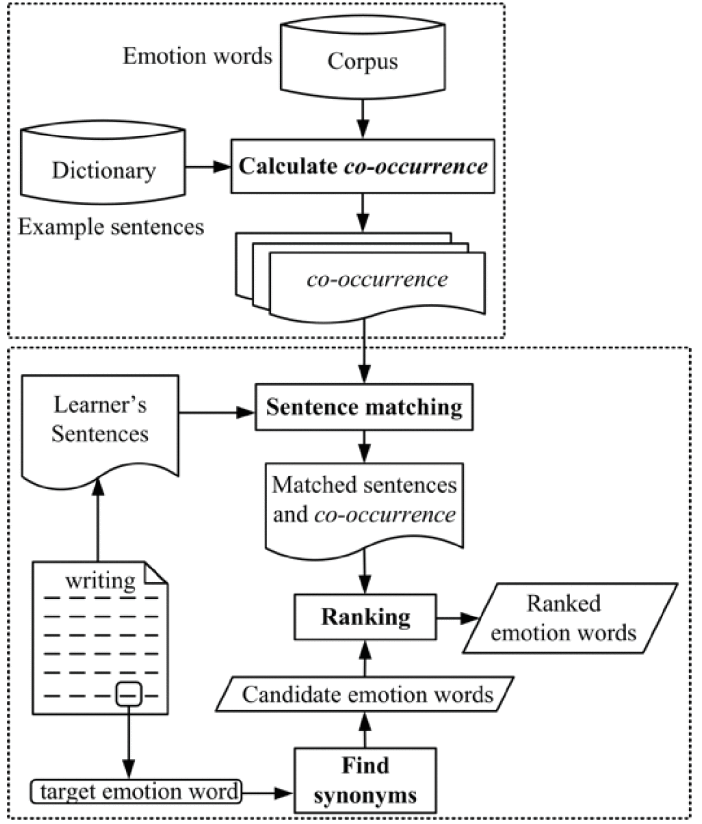
\includegraphics[height=11.25cm,width=9cm]{Figure1.png}
\counterwithin{figure}{section}
\centering
\caption{Figure 1}
\end{figure}

\section{DEVELOPMENT OF RESOLVE}
To provide learners with technology support, a corpus was built and a writing assistance system was developed. 
\paragraph{}
Regarding the corpus, 1,000 emotion words from WordNet-Affect were first collected. Next, to increase coverage, 2,785 synonyms of the above emotion words were included from WordNet Synset and the Merriam Webster Dictionary. Then, following classification of the emotion words used in WordNet Affect, all 3,785 emotion words were categorized into six major emotion categories: anger, disgust, fear, joy, sadness, and surprise, which is the most used characterization in many studies. 
\paragraph{}
The RESOLVE system was developed adopting machine learning techniques because of its strength of learning from data and making predictions, which is an effective approach to sentiment analysis or opinion mining. Figure 1 shows the RESOLVE framework. We first extracted approximately 2.8 million example sentences from Vocabulary.com and calculated the co-occurrences of all 3,785 emotion words and these example sentences. The purpose of this was to determine the appropriateness of the emotion words for the example sentences. At runtime, the synonyms of the target emotion word in the learner context are collected from Word- Net Synset. Next, each sentence in the learner context is compared with the sentences in Vocabulary.com using the edit distance algorithm, which quantifies the similarity between two word sequences as the number of steps it takes to trans- form one into the other. As a result, those sentences in the dictionary that share the highest similarity with those in the learner writings are then selected. Based on the co-occurrence of the collected synonymous emotion words and the selected sentences from the dictionary, the sorting algorithm ranks the synonyms. As a result, the suggested emotion words are context-aware instead of being listed in an alphabetical order. It is worth noting that given more detailed contextual clues, the algorithm can effectively specify the emotion. However, longer contexts and more synonyms would increase computational complexity. 

\begin{figure}[H]
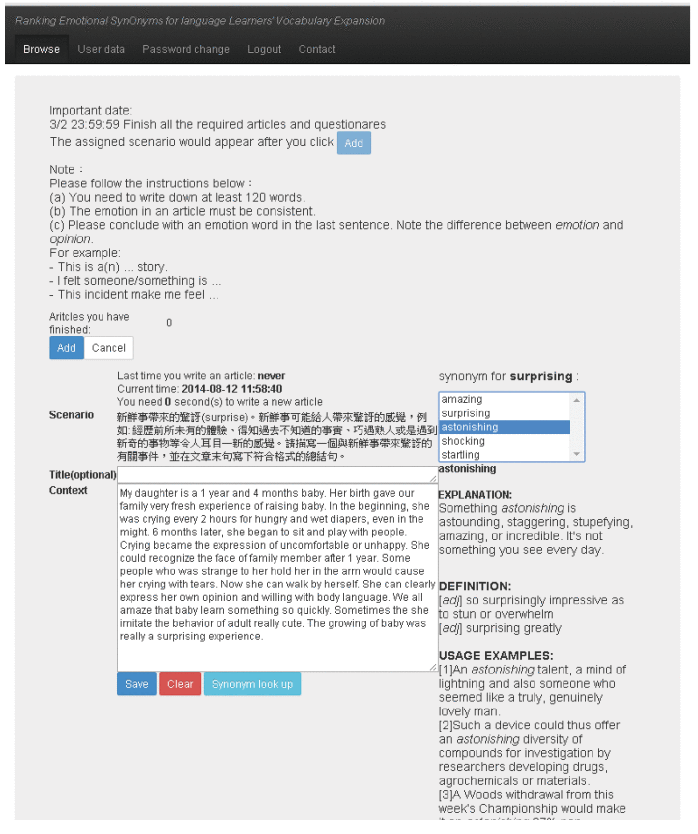
\includegraphics[height=12.5cm,width=10.46cm]{Figure2.png}
\counterwithin{figure}{section}
\centering
\caption{Figure 2}
\end{figure}

\paragraph{}
To prevent the context-switching problem, the RESOLVE interface (Figure 2) consists of a writing area on the left and a reference area on the right. Once the learner finishes writing, he may highlight the target emotion word surprising and click the synonym look up button. On receiving this request, the system initializes four zones on the right: synonyms for surprising, explanation of how the word can be used, definition, and usage examples. The listed emotion synonyms are amazing, surprising, astonishing, shocking, and startling, which are ranked based on the given context. This synonym ranking suggests the extent of their appropriateness. In this case amazing is deemed more appropriate than startling. Note that the suggested synonyms may include the target word. 
\paragraph{}
If the learner selects one of the synonyms, such as astonishing, the system returns the corresponding usage information, including the descriptions of the specific scenarios, definitions, and example sentences. Such information illustrates how the emotion word could be used, which enables learners to differentiate nuances of emotion words and select appropriate emotion words to fit their contexts. In this way, the suggested synonyms are customized for individual learners. 

\section{THE EVALUATION STUDY}
To assess the system’s effectiveness, an evaluation study was conducted. Note that the research materials and experimental procedures were pilot tested. 

\subsection{Participants}

Thirty-six volunteers were recruited online to participate in this experiment. They confirmed their willingness to participate in this study by signing a consent form. Because three participants were unable to fully participate in all of the experimental activities, data of a total of 33 participants were valid for analysis. These participants, 24 females and nine males, were aged between 23 and 38 (mean age 28.4). They were all Mandarin-speaking EFL learners with educational backgrounds of undergraduate or higher. Eight of them majored in English in college whereas 25 of them were non-English majors. The participants had at least six years of formal English instruction and were estimated as upper intermediate learners of English, as measured by the proficiency test they took at the beginning of the experiment. A non-experimental pre- and post-test design was conducted. Grounded in the statistical analyses, the findings are presented below. 

\begin{figure}[H]
\includegraphics[height=5cm,width=10cm]{Table1.png}
\counterwithin{figure}{section}
\centering
\caption{Table 1}
\end{figure}

\subsection{Research Materials}
\paragraph{}
A writing task and a survey questionnaire were developed to evaluate whether learners benefitted from the proposed system. The purpose of this study is to investigate learners’ general performance in emotion word use. Thus, Ekman’s six emotion categories was adopted, the most used characterization in many previous studies, while designing the writing task. For each category, we designed three individual scenarios, which were determined based on the results of a pilot study. The scenarios, described in the participants’ first language to avoid misunderstandings, were to illustrate the emotion category instead of suggesting a specific emotion word. Table 1 exemplifies scenarios for anger and disgust. The participants were allowed to decide their own events relevant to the given scenarios. Also, they were to express a consistent emotion through the whole writing in at least 120 words and use a specific emotion word to describe their feelings. 
\paragraph{}
In addition, a seven-item reflection questionnaire was developed to elicit participant opinions on RESOLVE. The first two questions sought information on participant writing behaviour and demands for tool support. The next four questions explored participant views on the system’s experiences in terms of system usability, the quality and number of suggested emotion synonyms, and usage information. The last question elicited participant perceptions on context-aware emotion vocabulary learning. All the questions used the five-point Likert agreement scale ranging from 1 (strongly disagree) to 5 (strongly agree). 

\subsection{Data Collection Procedure}
A pilot test was conducted three months before the experiment to identify the feasibility and effectiveness of the operational procedure. A group of 19 EFL college students enrolled in an English writing course participated in a five-week experiment involving the RESOLVE system. We thereafter revised the experimental design based on these preliminary results. The study was conducted outside of class time and lasted for five weeks: 
\paragraph{}
\textbf{Pre-test:} At the beginning of the study, the participants took an English proficiency test. Afterwards, they were evenly divided into six groups according to their proficiency test scores. Then the six categories were randomly assigned to the six groups. All the participants completed a writing task based on the second scenario of the assigned emotion categories. 
\paragraph{}
\textbf{Treatment:} During the three-week treatment phase, each participant was required to complete a total of nine writings for three scenarios of the assigned emotion category on the RESOLVE system. Precisely, three writings for one assigned scenario had to be completed per week. The participants were allowed to decide the events relevant to the given scenarios. After reviewing the synonymous emotion words and the corresponding usage information, the learner could either select one of the suggested emotion words or keep his original one to describe his feeling. Note that in order to maintain the quality of learning, the interval between any two writings from the same participant was at least 24 hours. 
\paragraph{}
\textbf{Post-test:} In the post-test, all the participants were to complete another writing task on the second scenario of their assigned emotion categories. They also filled in the survey questionnaire. 
\paragraph{}
Several issues are worth noting. First, the second scenario was determined to avoid the effect of short-term memory mainly because the writing task of scenario two was per- formed in the third week, which was not too close to either the pre-test week or the post-test week. Second, the events they described in the pre- and post-tests were identical. The purpose was to compare the appropriateness of the emotion words the participants produced. Third, the participants were unable to refer back to their previous writings, which discouraged them from copying the previous writings. Note that on both the pre- and post-tests, the participants completed their writings using the RESOLVE interface but with the suggestion of synonymous emotion words withheld. 
\subsection{Design of Scoring Criteria}
To evaluate the appropriateness of learners’ emotion word use, a 7-point grading scale ranging from 0 (the least appropriate) to 6 (the most appropriate) was used. Two native- speaker judges, trained before the pilot study, were given the participants’ pre-and post-writings as well as the lists of synonyms of the target emotion words they produced, which were extracted from the corpus. The judges gave scores to each emotion synonym on the lists based on the participants’ contexts. Note that the judges had no information about the target emotion words participants produced in both the pre-and post-writings, which avoided scoring bias. Participants’ word choice rather than grammatical accuracy was the focus in the evaluation. If two or more words were considered equally appropriate, they were given equal scores. A weighted Cohen’s Kappa value of 0.68 indicated substantial agreement between the judges. 
\section{RESULTS AND DISCUSSION}
The current study investigates whether and to what extent RESOLVE helped language learners with emotion word use. We examined learner emotion word use in the pre- and post-writings as well as analysed their reflections of RESOLVE experience. To reflect learner performance accurately, the results of the two judges’ evaluations on each issue were reported respectively. 
\subsection{Tool Effectiveness on Learner Use of Emotion Words}
The first research question investigated whether learners benefitted from the proposed tool support. To answer this question, we compared learners’ scores of their emotion word use in the pre-and post-writings. Besides the gain scores, we also reported learners’ error reduction ratios (ERR) in order to avoid analytical bias. 

\begin{figure}[H]
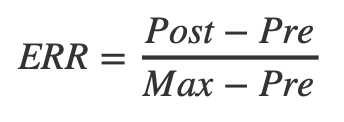
\includegraphics[height=2cm,width=6cm]{Equation.png}
\counterwithin{figure}{section}
\centering
\caption{Equation}
\end{figure}

\paragraph{}
The error reduction ratio (ERR) quantifies the learner’s error reduction from the pre-test to the full mark, which is shown in above equation. where Max is the full mark (six in our scoring scheme), Post and Pre are the scores of post- and pre-tests, respectively. This can be interpreted as a measure of the room for improvement. Note that errors in this study indicate inappropriate emotion word use. Taking this study as an example, two learners both improved their scores by 1 point (out of 6): one learner’s score increased from 4 to 5; the other from 5 to 6. Their improvements were 20.0% ((5−4)/5) and 16.7% ((6−5)/6) respectively. At first sight, the learner who scored higher at first did not make as significant progress as the lower-scoring learner. Indeed, to a certain extent, it can be hard for learners with better initial performance to make considerable improvements. However, the ERR shows different results. The improvement of the initially lower-scoring learner is 50.0% ((5−4)/(6−4)) while that of the initially higher-scoring learner is 100.0% ((6−5)/(6−5)). Because ERR provides us with an alternative view on learners’ improvement, we included ERR to examine participants’ performances. The two judges’ scorings were reported individually, which helped us learn the different views they held on learners’ emotion word use. 
\paragraph{}
We first compared learners’ average scores in the pre- and post-tests. The first row of Table 2 shows that all learners achieved expected gains. ANOVA results revealed that there was a significant difference between learner performance on the pre-test and post-tests (Judge 1: F(1,64)= 9.67, p value=0.003 and Judge 2: F (1,64)= 9.92, p value=0.002). This indicates that the participants made improvement on emotion word use after the three-week treatment. 

\begin{figure}[H]
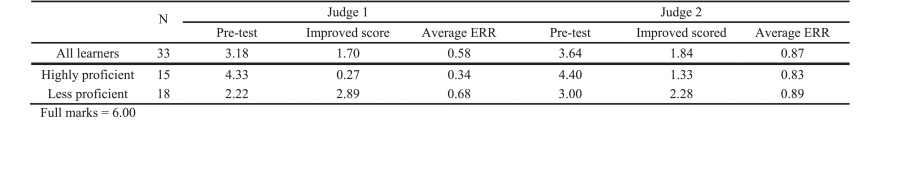
\includegraphics[height=3cm,width=15cm]{Table2.png}
\counterwithin{figure}{section}
\centering
\caption{Table 2}
\end{figure}

\begin{figure}[H]
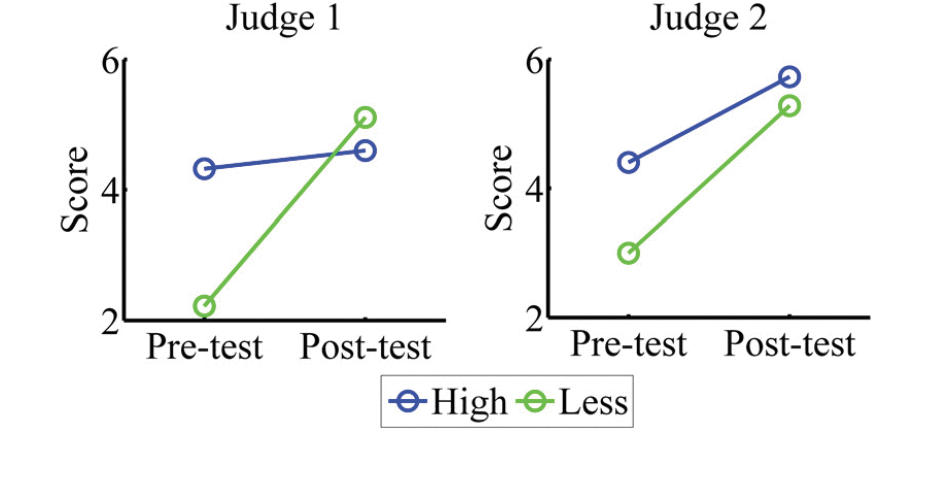
\includegraphics[height=8cm,width=16cm]{Figure3.png}
\counterwithin{figure}{section}
\centering
\caption{Figure 3}
\end{figure}

\paragraph{}
Next, we investigated whether RESOLVE was of great benefit to different learners (Table 2, second panel). To do so, the participants were divided into two groups based on their scores of the proficiency test, which was conducted in the first week. A total of 15 participants scored above or equal to the grand average (67.45), so they were classified as highly proficient. The other 18 participants with below-average scores were classified as less proficient. The average scores of the highly and less proficient groups were 80.93 and 56.22 out of 100.00 respectively. The learning effectiveness of the highly and less proficient students is visualized in Figure 3. Both figures showed that after the treatment, less proficient students made more noticeable improvement as compared with the highly proficient students. In fact, less proficient students achieved almost the same or even higher levels of performance in the emotion wording task than their counterparts. 
\paragraph{}
The significance of the improvements of both groups was further quantified by ANOVA: the first judge’s evaluation showed a significant difference between both the highly and less proficient learners (F(1, 31)=9.76, p value=0.004), whereas according to the second judge, no significant difference existed between the two groups (F(1, 31)=.71, p value=0.405). To understand whether less proficient learners benefited from the tool support, or highly proficient learners’ higher scores in the pre-test limited their potential for improvements, we calculated learner error reductions. Clearly, the ERRs of the less proficient learners were higher than those of the highly proficient learners based on both judges’ evaluations. It indicates that the less proficient learners made significant progress even after the error residual was normalized despite insignificant difference between the two groups in the second judge’s view. Since the results revealed that the less proficient learners showed greater improvements, we further sought to investigate how the performance of these two groups differed, which is discussed in the next section. 
\subsection{Performance Comparison of Learners}
\paragraph{}
The second research question attempted to explore how the improvements of highly and less proficient learners differed. A second order polynomial curve was used to fit these (proficiency level, improved score) data points: the trend is shown in Figure 4. From the first judge’s evaluation (left subfigure), a negative relationship can be seen between the learners’ language proficiency and their improved scores. In other words, the lower the proficiency level, the more improvement achieved by the participant. The second judge’s view, however, was somewhat different. The right figure reveals a downward trend for highly proficient learners and a slightly upward trend for less proficient learners. This means that for the highly proficient group, the higher the proficiency level, the smaller the gain; however, the less proficient learners did not follow this pattern. 
\paragraph{}
Taken together, the judges shared similar opinions with respect to the performance of the highly proficient learners whereas there were discrepancies for the less proficient learners. To investigate these differences, we scrutinized the individual performances of the less proficient participants. Discrepancies were found in four less proficient participants, so the data of these four participants were particularly examined. Table 3 shows the breakdown of the participants’ emotion words and their scores in the pre- and post-tests. 

\begin{figure}[H]
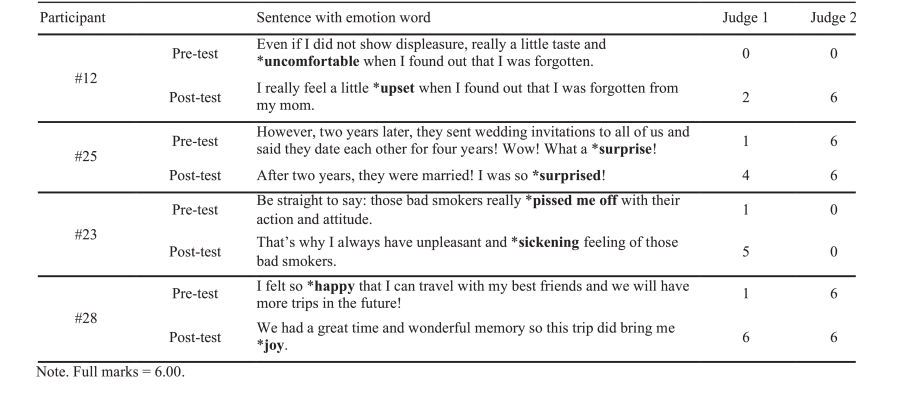
\includegraphics[height=7cm,width=16cm]{Table3.png}
\counterwithin{figure}{section}
\centering
\caption{Table 3}
\end{figure}

\paragraph{}
Specifically, from the perspective of Judge 1, these four participants showed improvements whereas from Judge 2’s view, no one made progress except Participant 1. Although both judges agreed on Participant 1’s improvement, they were not consistent about the appropriateness of his emotion word use. We then take a further look at the performance of the other three participants from the evaluation of Judge 2. Participant 2 and Participant 4 received full marks in the pre- and post-tests, leaving no room for improvement. Turning to Participant 3, the zero point in both pre- and post-tests showed that his emotion words were the least appropriate. For this reason, the views of both judges differed greatly. Researchers such as Dewaele and Pavlenko suggest that the use of emotion words is related to individual experience; this could explain the judges’ divergent views. 
\paragraph{}
If we exclude the markedly different data, a similar trend can be seen in the judge evaluations as that seen in Figure 5. That is, for the less proficient group, the lower the proficiency level, the greater the improvement. In contrast, for highly proficient participants, the higher the proficiency level, the smaller their gains. This could be because they had confidence in their command of emotion words, as evidenced by the fact that seven out of 15 participants used the same emotion words in their pre- and post-writings, which scored full marks. On the other hand, 16 out of 18 participants used different emotion words in their writings. Their improved scores showed that their attempts were successful. 
\paragraph{}
It is worth noting that for the participants whose English proficiency was extremely high or extremely low, the bene- fit of RESOLVE was less obvious. It is not surprising that advanced learners had sufficient competence to make appropriate lexical choices. On the other hand, the low-achieving learners’ limited vocabulary was likely to make emotion word learning much more demanding. Overall, less proficient learners significantly benefitted from the proposed system, RESOLVE, in emotion word learning compared with the highly proficient learners, which was expected. 

\vspace{2em}
\begin{figure}[H]
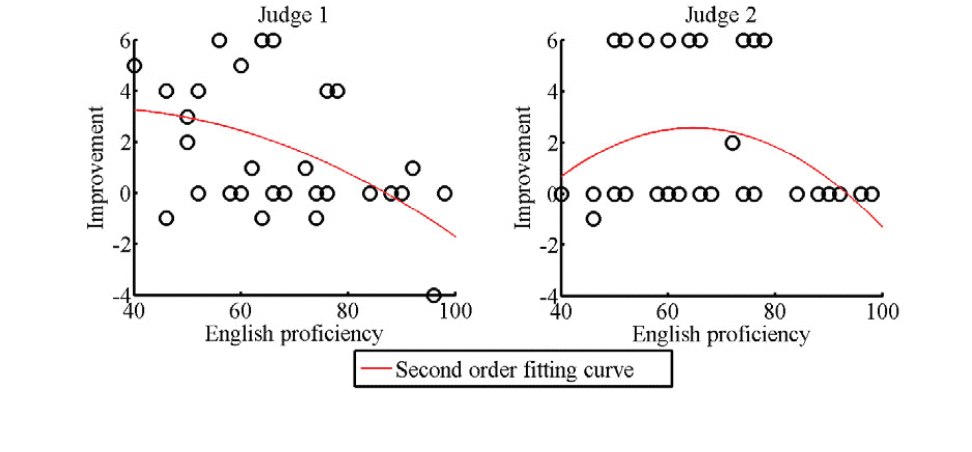
\includegraphics[height=8cm,width=16cm]{Figure4.png}
\counterwithin{figure}{section}
\centering
\caption{Figure 4}
\end{figure}


\begin{figure}[H]
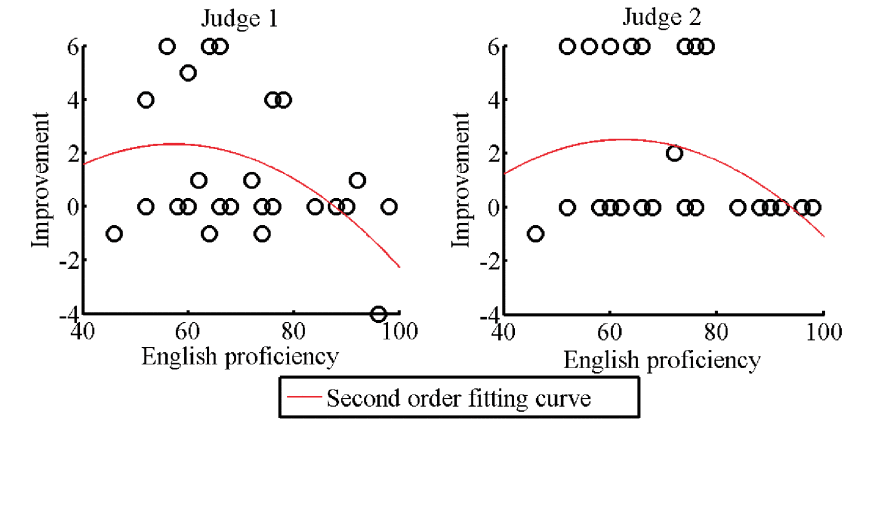
\includegraphics[height=8cm,width=16cm]{Figure5.png}
\counterwithin{figure}{section}
\centering
\caption{Figure 5}
\end{figure}

\subsection{Learners’ Perceptions of Context-Based Emotion Synonym Learning}
\paragraph{}
To answer this research question, a seven-item reflection questionnaire was designed to elicit participant perceptions on RESOLVE in terms of learner needs, system usefulness, and its contribution to language learning. Moreover, participants’ open-ended responses were collected to elicit the rea- sons underlying their answers to each closed-form question. To have a greater understanding of the opinions of different students, the feedback of learners with different proficiency levels was analysed (Table 4). A two-sample t test was carried out, and the results showed no significant difference between the two groups’ responses. Learners’ perceptions on each survey question were discussed below. 
\paragraph{}
The first panel illustrates the participant learning back- grounds: their writing behaviour (item 1) and their needs for tool support (item 2). The scores of these two items were quite high (all above 3.80/5.00). Both groups reported that they intended to restate their feelings. To have a better under- standing of the behaviour of the two groups, we scrutinized the emotion words produced by the participants and found that eight highly and 16 less proficient participants used different emotion words in their pre- and post-writings. It is likely that highly proficient participants had greater confidence in their emotion word use than the less proficient ones. Meanwhile, participants’ strong demand for tool support indicated that learners needed help to be engaged in emotion word learning. 
\paragraph{}
The second panel shows participant perceptions on system usefulness, including system function (item 3) and suggested information (item 4-6). First, the tool usability scored quite high. In particular, both groups were satisfied with being able to consult synonyms and usage information directly without switching visual focus between webpages while composing their writing. The results supported previous research on the split-attention effect: Learning in an integrated environment reduces mental effort and improves learning results. Participants’ feedback showed that our design met their needs. Second, the information provided by RESOLVE included the ranked emotion words (item 4), the number of synonymous emotion words (item 5), and the usage information (item 6). Both groups appreciated the suggested emotion words as well as the usage information. Less proficient learners particularly acknowledged that the usage information (i.e., scenario descriptions, definitions and example sentences), benefit them in learning to use emotion synonyms appropriate to their contexts. Interestingly, both groups did not seem to share similar views on the number of suggested synonyms, even though there was no significant difference between them. Less proficient learners appreciated five suggestions whereas highly proficient participants expected more suggestions. Some participants suggested that eight synonyms would yield adequate choices for better wording. 
\paragraph{}
The last question (item 7) sought participant reflections on the role of RESOLVE for language proficiency. Nearly 80\% of the learners (26 out of 33 participants) saw RESOLVE as a practical reference aid that benefited their writing and promoted language competence. A significantly higher number of less proficient learners (n=16) acknowledged the tool assistance. The opinions of the less proficient participants echoed the findings of the previous research questions that they received greater benefit from the tool support than their counterparts. 

\begin{figure}[H]
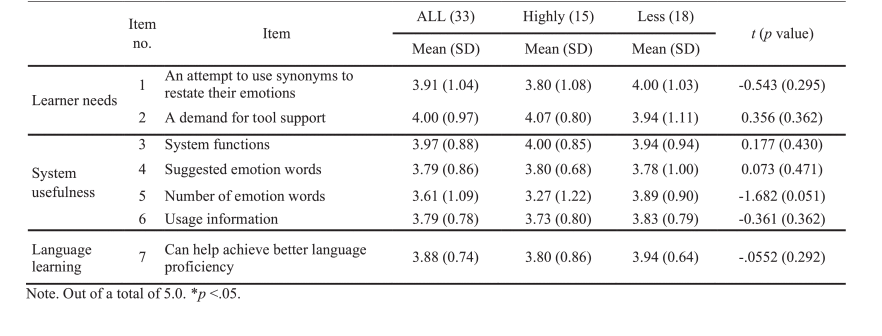
\includegraphics[height=11.25cm,width=9cm]{Table4.png}
\counterwithin{figure}{section}
\centering
\caption{Table 4}
\end{figure}

\section{CONCLUSION}
\paragraph{}
Emotion vocabulary has been an important concern in several disciplines. They were especially widely used in sentiment detection or prediction. However, it has not received particular attention in foreign language teaching and learning. In view of the paucity of research, we developed RESOLVE, a context-based emotion synonym suggestion system. Developed using machine learning techniques, RESOLVE is capable of suggesting contextually appropriate emotion synonyms. The usage information is also provided to reinforce learner’s word use. The tool effective- ness was assessed using a writing task and a reflection questionnaire. The results demonstrated that both the suggested emotion synonyms and the corresponding usage information are beneficial to learners’ use of emotion vocabulary. Notably, less proficient participants showed greater improvements. Moreover, analysis of the questionnaire responses showed that the participants appreciated the tool support in learning appropriate emotion word use. 
\subsection{Pedagogical Implications}
Mastering emotion words is a challenging task for language learners, so emotion vocabulary should be explicitly taught and consciously learned. The RESOLVE system is applicable for use in classroom teaching and activities. The approach proposed in this study could be replicated in the classroom. Instructors could create various scenarios for specific emotion categories and have their students compose writings via consulting RESOLVE. Afterwards, instructors elaborate on how the words students produce could be used in various scenarios. Such pedagogical activities enable learners to develop a clearer understanding of as well as stronger command of emotion word use. 
\subsection{Limitations and Future Work}
To the best of our knowledge, this is the first study considering the application of sentiment analysis to assisting language learning. It is worth mentioning that although the focus of the current study is emotion vocabulary learning, the RESOLVE system can be easily adapted for other vocabulary or synonym learning. While the preliminary findings supported that the developed system was beneficial to emotion word use, there are limitations in this study that could be improved. For example, a greater number of participants should be involved, which could help us take a closer look at potential learner difficulties in the use of emotion words. Also, tool comparison (e.g., online thesauri) could be conducted to examine their individual impacts on learners. 

\newpage
\cleardoublepage
% \addcontentsline{toc}{section}{\textbf{References}}
\addcontentsline{}{section}{\textbf{References}}
\begin{thebibliography}{9}


\bibitem{d} J. Altarriba, ‘‘Emotion, memory, and bilingualism,’’ in \emph{Foundations of Bilingual Memory, }J. Altarriba and R. Heredia, Eds. New York, NY, USA: Springer, 2014, pp. 185–203.
\bibitem{d} A. Pavlenko, ‘‘Affective processing in bilingual speakers: Disembodied cognition?’’ \emph{ “Int. J. Psychol., }vol. 47, no. 6, pp. 405–428, 2012.
\bibitem{d} G. L. Clore and A. Ortony, ‘‘The semantics of the affective lexicon,’’ in \emph{Cognitive Perspectives on Emotion and Motivation. }New York, NY, USA: Springer, 1988, pp. 367–397.
\bibitem{d} E. H. Hovy, ‘‘What are sentiment, affect, and emotion? Applying the methodology of Michael Zock to sentiment analysis,’’ in \emph{Language Production, Cognition, and the Lexicon, }N. Gala, R. Rapp, and G. Bel-Enguix, Eds. Cham, Switzerland: Springer, 2015, pp. 13–24.
\bibitem{d} A.PavlenkoandV.Driagina,‘‘RussianemotionvocabularyinAmerican learners’ narratives,’’ \emph{Modern Lang. J., }vol. 91, no. 2, pp. 213–234, 2007.
\bibitem{d} C.-C. Huang and L.-W. Ku, ‘‘Interest analysis using semantic PageRank and social interaction content,’’ in \emph{Proc. IEEE 13th Int. Conf. Data Mining Workshops, }Dec. 2013, pp. 929–936.
\bibitem{d} P.-Y.Lu,Y.-Y.Chang,andS.-K.Hsieh,‘‘Causingemotionincollocation: An exploratory data analysis,’’ in \emph{Proc. 25th Conf. Comput. Linguistics Speech Process.,} 2013, pp. 236–249.
\bibitem{d} B.Pang,L.Lee,andS.Vaithyanathan,‘‘Thumbsup?:Sentiment classification using machine learning techniques,’’ in \emph{Proc. ACL Conf. Empirical Methods Natural Lang. Process.,} 2002, pp. 79–86.
\bibitem{d} J.-M. Dewaele, ‘‘Investigating the psychological and emotional dimensions in instructed language learning: Obstacles and possibilities,’’ \emph{Modern Lang. J.,} vol. 89, no. 3, pp. 367–380, 2005.
\bibitem{d} J.-M.Dewaele and A.Pavlenko,‘‘Emotionvocabularyininterlanguage,’’ \emph{Lang. Learn.,} vol. 52, no. 2, pp. 263–322, 2002.
\bibitem{d} T.Kaneko,‘‘Hownon-nativespeakersexpressanger,surprise,anxiety and grief: A corpus-based comparative study,’’ in \emph{Proc. Corpus Linguistics Conf.,} 2003, pp. 384–393.
\bibitem{d} E. M. Rintell, ‘‘That’s incredible: Stories of emotion told by second language learners and native speakers,’’ \emph{Developing Communicative Competence in a Second Language.} 1990, pp. 75–94.
\bibitem{d} J.-M. Dewaele, ‘‘On emotions in foreign language learning and use,’’ \emph{Lang. Teacher,} vol. 39, no. 3, pp. 13–15, 2015.
\bibitem{d} C. R. Graham, A. W. Hamblin, and S. Feldstein, ‘‘Recognition of emotion in English voices by speakers of Japanese, Spanish and English,’’ \emph{Int. Rev. Appl. Linguistics Lang. Teach.,} vol. 39, no. 1, pp. 19–37, 2001.
\bibitem{d} Y. Yeh, H.-C. Liou, and Y.-H. Li, ‘‘Online synonym materials and concor- dancing for EFL college writing,’’ \emph{Comput. Assist. Lang. Learn.,} vol. 20, no. 2, pp. 131–152, 2007.
\bibitem{d} M. Martin, ‘‘Advanced vocabulary teaching: The problem of synonyms,’’ \emph{Modern Lang. J.,} vol. 68, no. 2, pp. 130–137, 1984.
\bibitem{d} D. Liu, ‘‘Salience and construal in the use of synonymy: A study of two sets of near-synonymous nouns,’’ \emph{Cognit. Linguistics,} vol. 24, no. 1, pp. 67–113, 2013.
\bibitem{d} D. Liu and S. Zhong, ‘‘L2 vs. L1 use of synonymy: An empirical study of synonym use/acquisition,’’ \emph{Appl. Linguistics,} vol. 37, no. 2, pp. 239–261, Apr. 2016.
\bibitem{d} W.-F. Chen, M.-H. Chen, and L.-W. Ku, ‘‘Embarrassed or awkward? Ranking emotion synonyms for ESL learners’ appropriate wording,’’ in \emph{Proc. 10th Workshop Innov. NLP Building Educ. Appl.,} 2015, pp. 144–153.
\bibitem{d} W.-F. Chen, M.-H. Chen, M.-L. Chen, and L.-W. Ku, ‘‘A computer- assistance learning system for emotional wording,’’ \emph{IEEE Trans. Knowl. Data Eng.,} vol. 28, no. 5, pp. 1093–1104, May 2016.
\end{thebibliography}
\end{document}